\documentclass[a4paper,11pt,dvipdfmx]{ujarticle}
% パッケージ
\usepackage{graphicx}
\usepackage{url}
% レイアウト指定を記述したファイルの読み込み
\input{layout}

% タイトルと氏名を変更せよ.
\title{日本におけるデジタル化の状況}
\author{G584362025 黒澤 歩夢}

\begin{document}

\maketitle %ここにタイトルが入る

\section{ブロードバインドの整備状況}
OECDによるブロードバインド回線調査\cite{oecd}によると,
図\ref{fig:加入者数}に示すように,
日本における100あたりのモバイルブロードバンドの加入者数は190.5で,第1位になっている.
2位エストニアで,3位米国と続く.

\begin{figure}[htbp]
    \centering
    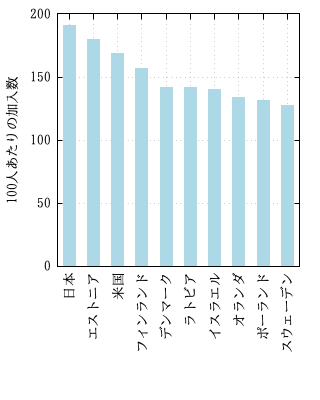
\includegraphics[width=0.6\linewidth]{fig21.png}
    \caption{光ファイバー回線の加入者数(100人あたり)}\label{fig:加入者数}
\end{figure}

\section{デジタル競争力ランキング}

国際経営開発研究所(IMD)の調査\cite{imd}によると,
表\ref{tbl:利用状況}に示すように,
日本のデジタル競争力のランキングは調査対象の64カ国中,総合で28位,知識分野で25位となっている.

\begin{table}[htbp]
    \centering
    \caption{デジタル競争力ランキング}
    \label{tbl:利用状況}

    \begin{tabular}{|l|r|r|}
        \hline
        国 & 総合 & 知識 \\
        \hline
        米国 & 1位 & 3位 \\
        \hline
        香港 & 2位 & 5位 \\
        \hline
        スウェーデン & 3位 & 2位 \\
        \hline
        デンマーク & 4位 & 8位 \\
        \hline
        シンガポール & 5位 & 4位 \\
        \hline
        \hline
        韓国 & 12位 & 15位 \\
        \hline 
        中国 & 15位 & 6位 \\
        \hline
        \hline
        日本 & 28位 & 25位 \\
        \hline
    \end{tabular}
\end{table}

\section{考察}
\begin{itemize}
    \item ブロードバンドの整備状況とデジタル競争力には相関はない。
    \item 米国は高い水準でデジタル化が行われている。
\end{itemize}
% ーーー
% ここから本文
% 節見出し: \section{}
% を使う

% 本文(1)
%  参考文献の参照: \cite{}
%  図番号の参照: \ref{}
% を使う
% 文献データベースのキーワードは oecd と imd
% になっている.

% 図の挿入
% \includegraphics{}
% を
% \begin{figure}[htbp]
% \end{figure}
% で囲み
% \caption{}
% で図のタイトルを入れる.
% \label{}
% を使って図番号が参照できるようにする
% また,
% \centering
% で図が中央に来るようにする

% ーーー
% 節見出し(2)

% 本文(2)

% 表の挿入
% \begin{tabular}
% \end{tabular}    
% による表の記述を 
% \begin{table}[htbp]
% \end{table}
% で囲み
% \caption{}
% で表のタイトルを入れる.
% \label{}
% を使って表番号が参照できるようにする
% また,
% \centering
% で表が中央に来るようにする

% ーーー
% 見出し(3)
% 考察
%
% \begin{itemize}
% \end{itemize}
% を使って箇条書きで記述する

% ここに参考文献が入る
%

\bibliographystyle{junsrt}
\bibliography{exercise.bib}

\end{document}